\documentclass[border=3mm,tikz,preview]{standalone}
\usepackage[utf8]{inputenc}
\usepackage{amsmath,amssymb,amsfonts}
\usepackage{graphicx}
\usepackage{tikz}
\usetikzlibrary{shapes.geometric, arrows.meta, positioning, shadows, calc, fit, backgrounds}
\usepackage{xcolor}
\begin{document}

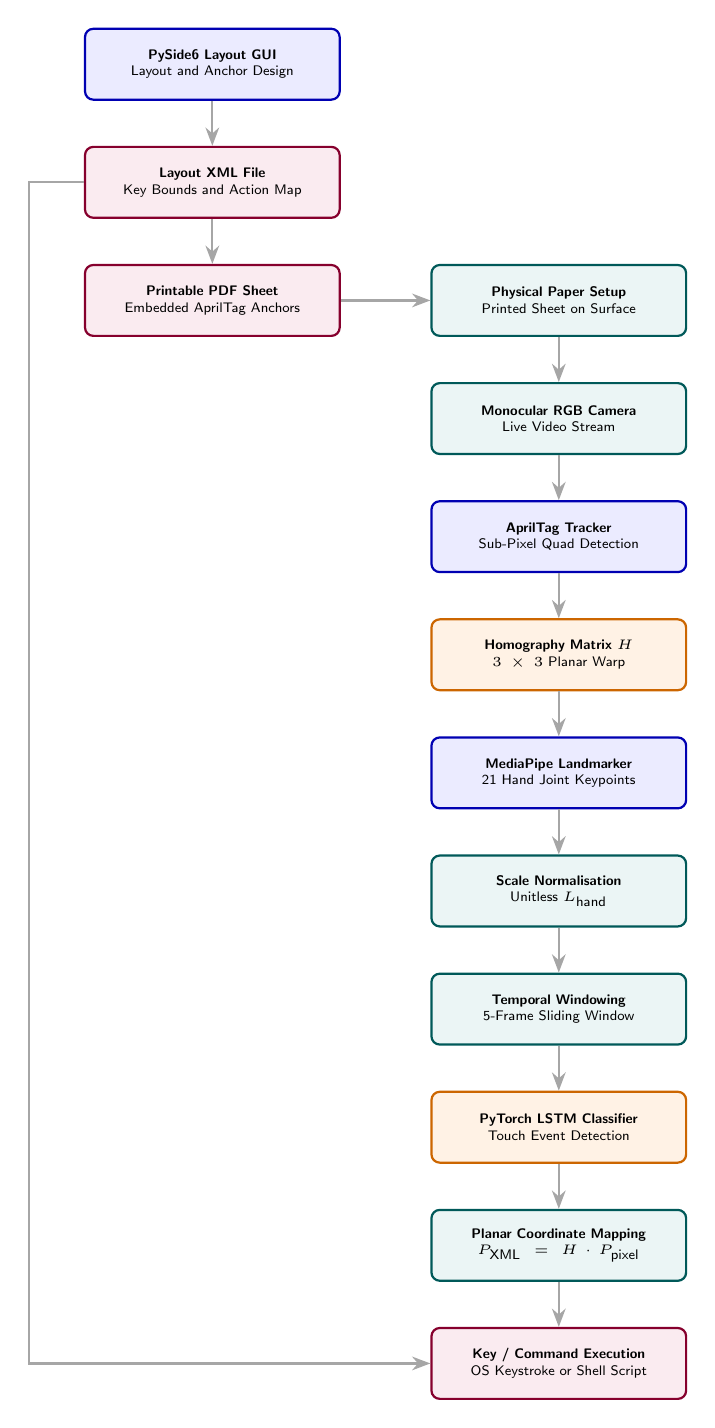
\begin{tikzpicture}[
    box/.style={draw=blue!70!black, rectangle, rounded corners=3pt,
                text width=3.0cm, minimum height=0.9cm, align=center,
                fill=blue!8!white, font=\sffamily\tiny, thick},
    process/.style={draw=teal!70!black, rectangle, rounded corners=3pt,
                text width=3.0cm, minimum height=0.9cm, align=center,
                fill=teal!8!white, font=\sffamily\tiny, thick},
    model/.style={draw=orange!80!black, rectangle, rounded corners=3pt,
                text width=3.0cm, minimum height=0.9cm, align=center,
                fill=orange!10!white, font=\sffamily\tiny, thick},
    artifact/.style={draw=purple!70!black, rectangle, rounded corners=3pt,
                text width=3.0cm, minimum height=0.9cm, align=center,
                fill=purple!8!white, font=\sffamily\tiny, thick},
    arrow/.style={-Stealth, thick, draw=gray!70}
]

%% ---- LEFT COLUMN: Offline Design Pipeline (x=0) ----
\node [box]      (designer)   at (0,  0)    {\textbf{PySide6 Layout GUI}\\Layout and Anchor Design};
\node [artifact] (xml)        at (0, -1.5)  {\textbf{Layout XML File}\\Key Bounds and Action Map};
\node [artifact] (pdf)        at (0, -3.0)  {\textbf{Printable PDF Sheet}\\Embedded AprilTag Anchors};

%% ---- RIGHT COLUMN: Online Runtime Pipeline (x=4.4) ----
\node [process]  (paper)      at (4.4, -3.0)  {\textbf{Physical Paper Setup}\\Printed Sheet on Surface};
\node [process]  (camera)     at (4.4, -4.5)  {\textbf{Monocular RGB Camera}\\Live Video Stream};
\node [box]      (apriltag)   at (4.4, -6.0)  {\textbf{AprilTag Tracker}\\Sub-Pixel Quad Detection};
\node [model]    (homography) at (4.4, -7.5)  {\textbf{Homography Matrix $H$}\\$3\times3$ Planar Warp};
\node [box]      (mediapipe)  at (4.4, -9.0)  {\textbf{MediaPipe Landmarker}\\21 Hand Joint Keypoints};
\node [process]  (norm)       at (4.4,-10.5)  {\textbf{Scale Normalisation}\\Unitless $L_{\text{hand}}$};
\node [process]  (window)     at (4.4,-12.0)  {\textbf{Temporal Windowing}\\5-Frame Sliding Window};
\node [model]    (lstm)       at (4.4,-13.5)  {\textbf{PyTorch LSTM Classifier}\\Touch Event Detection};
\node [process]  (mapping)    at (4.4,-15.0)  {\textbf{Planar Coordinate Mapping}\\$P_{\text{XML}}=H\cdot P_{\text{pixel}}$};
\node [artifact] (execution)  at (4.4,-16.5)  {\textbf{Key / Command Execution}\\OS Keystroke or Shell Script};

%% ---- LEFT COLUMN ARROWS (strictly top-to-bottom) ----
\draw [arrow] (designer) -- (xml);
\draw [arrow] (xml)      -- (pdf);

%% ---- BRIDGE: PDF to physical paper (horizontal, same y level) ----
\draw [arrow] (pdf.east) -- (paper.west);

%% ---- RIGHT COLUMN ARROWS (strictly top-to-bottom) ----
\draw [arrow] (paper)      -- (camera);
\draw [arrow] (camera)     -- (apriltag);
\draw [arrow] (apriltag)   -- (homography);
\draw [arrow] (homography) -- (mediapipe);
\draw [arrow] (mediapipe)  -- (norm);
\draw [arrow] (norm)       -- (window);
\draw [arrow] (window)     -- (lstm);
\draw [arrow] (lstm)       -- (mapping);
\draw [arrow] (mapping)    -- (execution);

%% ---- XML load feed (routes along far-left margin, no box crossings) ----
\draw [arrow] (xml.west) -- ++(-0.7,0) |- (execution.west);

\end{tikzpicture}

\end{document}
